\begin{center}
  \Large
  \textbf{BIOGRAFI PENULIS}
\end{center}

\addcontentsline{toc}{chapter}{BIOGRAFI PENULIS}

\vspace{2ex}

\begin{wrapfigure}{L}{0.3\textwidth}
  \centering
  \vspace{-3ex}
  % Ubah file gambar berikut dengan file foto dari mahasiswa
  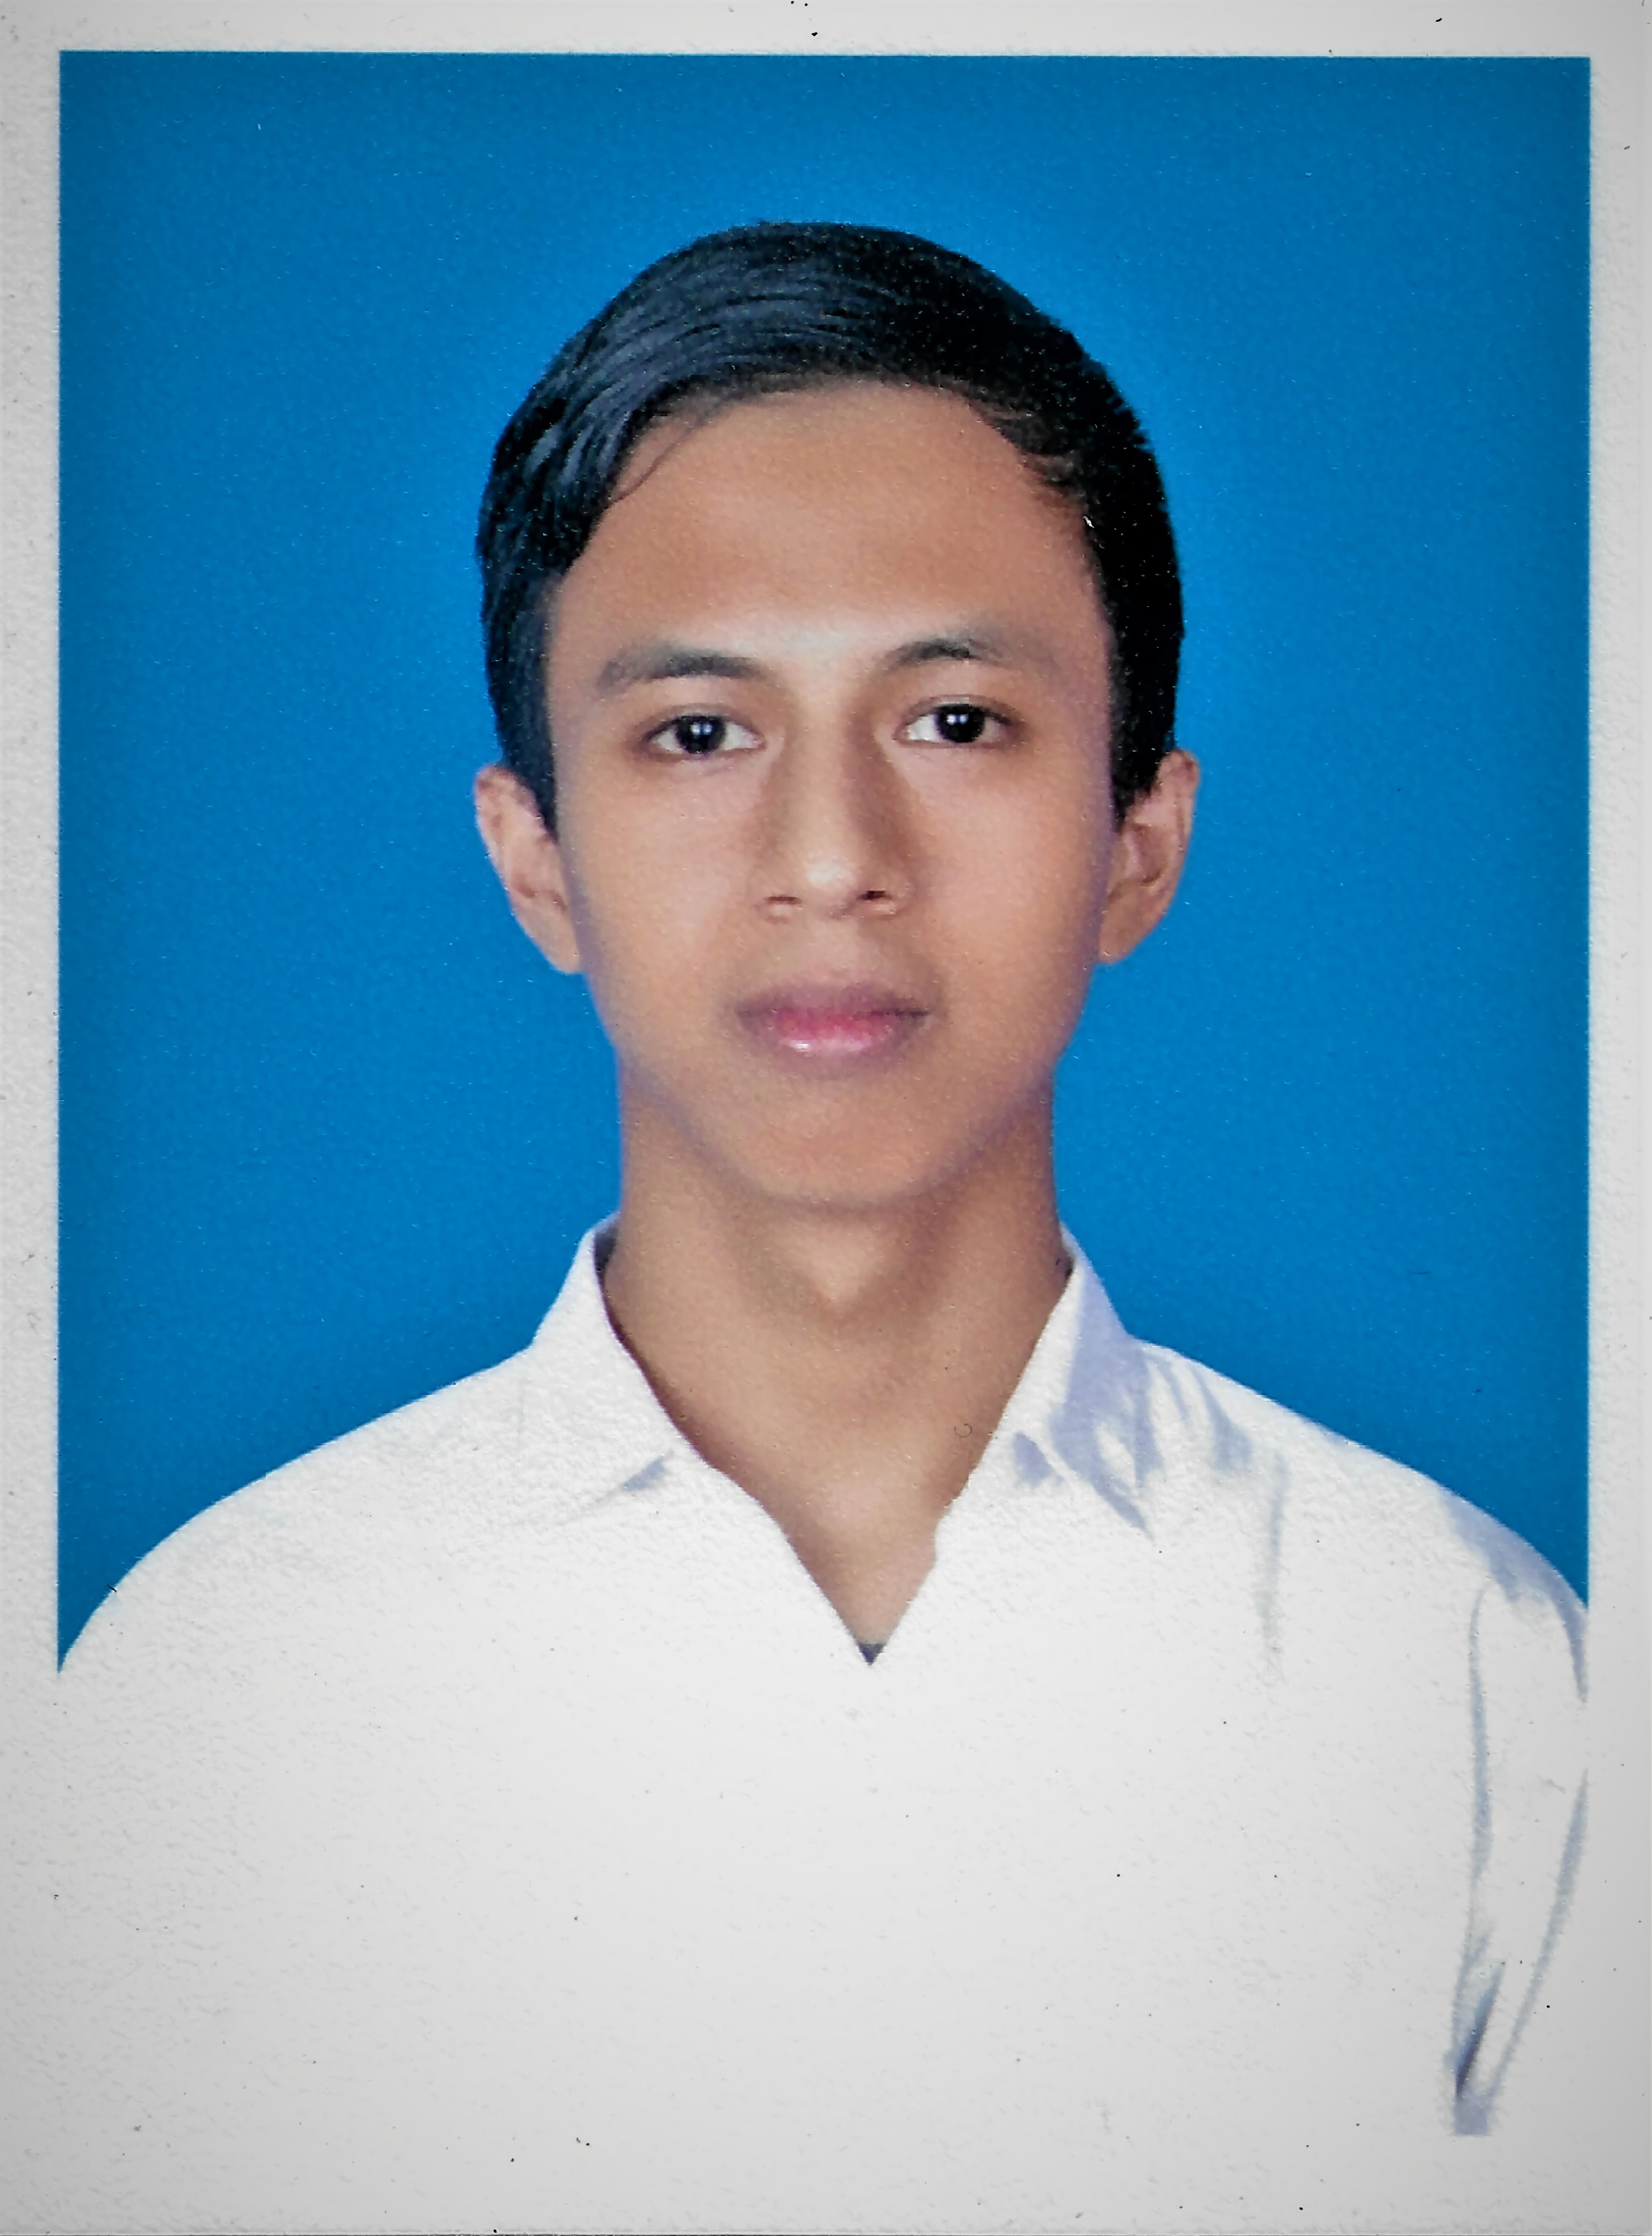
\includegraphics[width=0.3\textwidth]{gambar/fotoku2.png}
  \vspace{-4ex}
\end{wrapfigure}

% Ubah kalimat berikut dengan biografi dari mahasiswa
Habibul Rahman Qalbi, lahir di Padang, Sumatra Barat pada tanggal 6 Juli 1999. Merupakan anak pertama dari tiga bersaudara. Lulusan SMA Negeri 3 Kota Jambi, Penulis melanjutkan ke Jenjang Pendidikan Tinggi, Strata 1 (S1) di Departemen Teknik Komputer, Institut Teknologi Sepuluh Nopember (ITS) Surabaya. Dalam masa perkuliahannya, penulis tertarik dengan pengembangan Artificial Intelligence, Mobile Computing dan Embedded System. Selain itu, penulis juga aktif dalam kegiatan organisasi seperti Unit Kegiatan Mahasiswa Teater Tiyang Alit. Penulis juga hobi bereksperimen terutama dalam hal menyeduh kopi. Bagi pembaca yang memiliki kritik, saran, atau pertanyaan mengenai tugas akhir ini dapat menghubungi penulis melalui habi6799@gmail.com